\chapter{Project Management}
\label{Chapter:ProjectManagement}
Due to the extensive length and size of this project, consideration into how the project can be effectively
managed is very important to project success. The following sections will discuss the chosen design and development methodologies, providing justification for each choice and will also look at the risks affecting project progress and success.

\section{Design Approach}
The design approach adopted for system UI was be component-driven design. Component-driven design allowed more focus and thought to be given for each component. Choosing this design methodology is beneficial as it means components are designed independently of each other, and also means that designed components can be re-used in multiple applications. 

For algorithm design, an Agile approach was used. Agile methodologies provided flexibility when researching and designing chosen algorithms. Over the course of the project, numerous algorithms were considered and with the flexibility provided by this approach meant any required changes to algorithm design were prompt.

\section{Software Development Methodology}
Such an approach works extremely well with Agile development as each component can be designed, built and tested. Agile techniques were used due to their flexibility in handling evolving requirements. Due to the length of which the project would run, it was important to adopt an adaptive development methodology. Building the system using Agile techniques eases the integration of new system components, and increases the efficacy of unit testing. Another reason that the agile approach was chosen was that as the project is developed, issues will arise which may not have been accounted for previously. This would not have been possible through a plan driven approach such as waterfall which does not allow the modification of requirements once they've been set out and hence an agile approach is a good way of tackling these issues. 

One fact that must be brought to light is that agile methodologies do not focus on documentation as much as a plan driven approach. Due to documentation being part of the non-functional requirements of this project and a key aspect, a modified version of the agile approach, one where documentation is important, was used. In addition to this rapid prototype development was also employed due to the overlapping of development and testing as this allowed for quick prototype version of components to be created and tested which could then be improved based on the user feedback. To counteract the effects of reduced documentation, regular meetings were held with with project supervisor to ensure that project goals remained on track. Similarly, within the project group itself weekly meetings were held. Much like daily scrums, these meetings again reinforced project goals and provided a platform where next steps or progress blockers could be discussed.

\section{Project Timeline}
The proposed project timeline, composed during the project specification and visible in Figure \ref{fig:timeline} has remained largely unchanged. Given how the timeline was designed, providing generous float time to each activity, few minor changes have needed to be made from the original plan. To accommodate for the increased workload faced by team members in Term 2, work on the final report was delayed until March. Although this at first seems like a major delay, the 14 week period initially assigned for writing this report was purposefully made that large in the event of unforeseen circumstances. Subsequently, draft completion date and feedback cycles were also pushed back. The implementation for each algorithm ran longer than originally planned. This again did not affect the overall plan as these tasks were already overlapping and as each algorithm was implemented by a different team member, full task parallelisation meaning the completion date for the final algorithm was successfully met.

\begin{figure}[H]
  \centering
  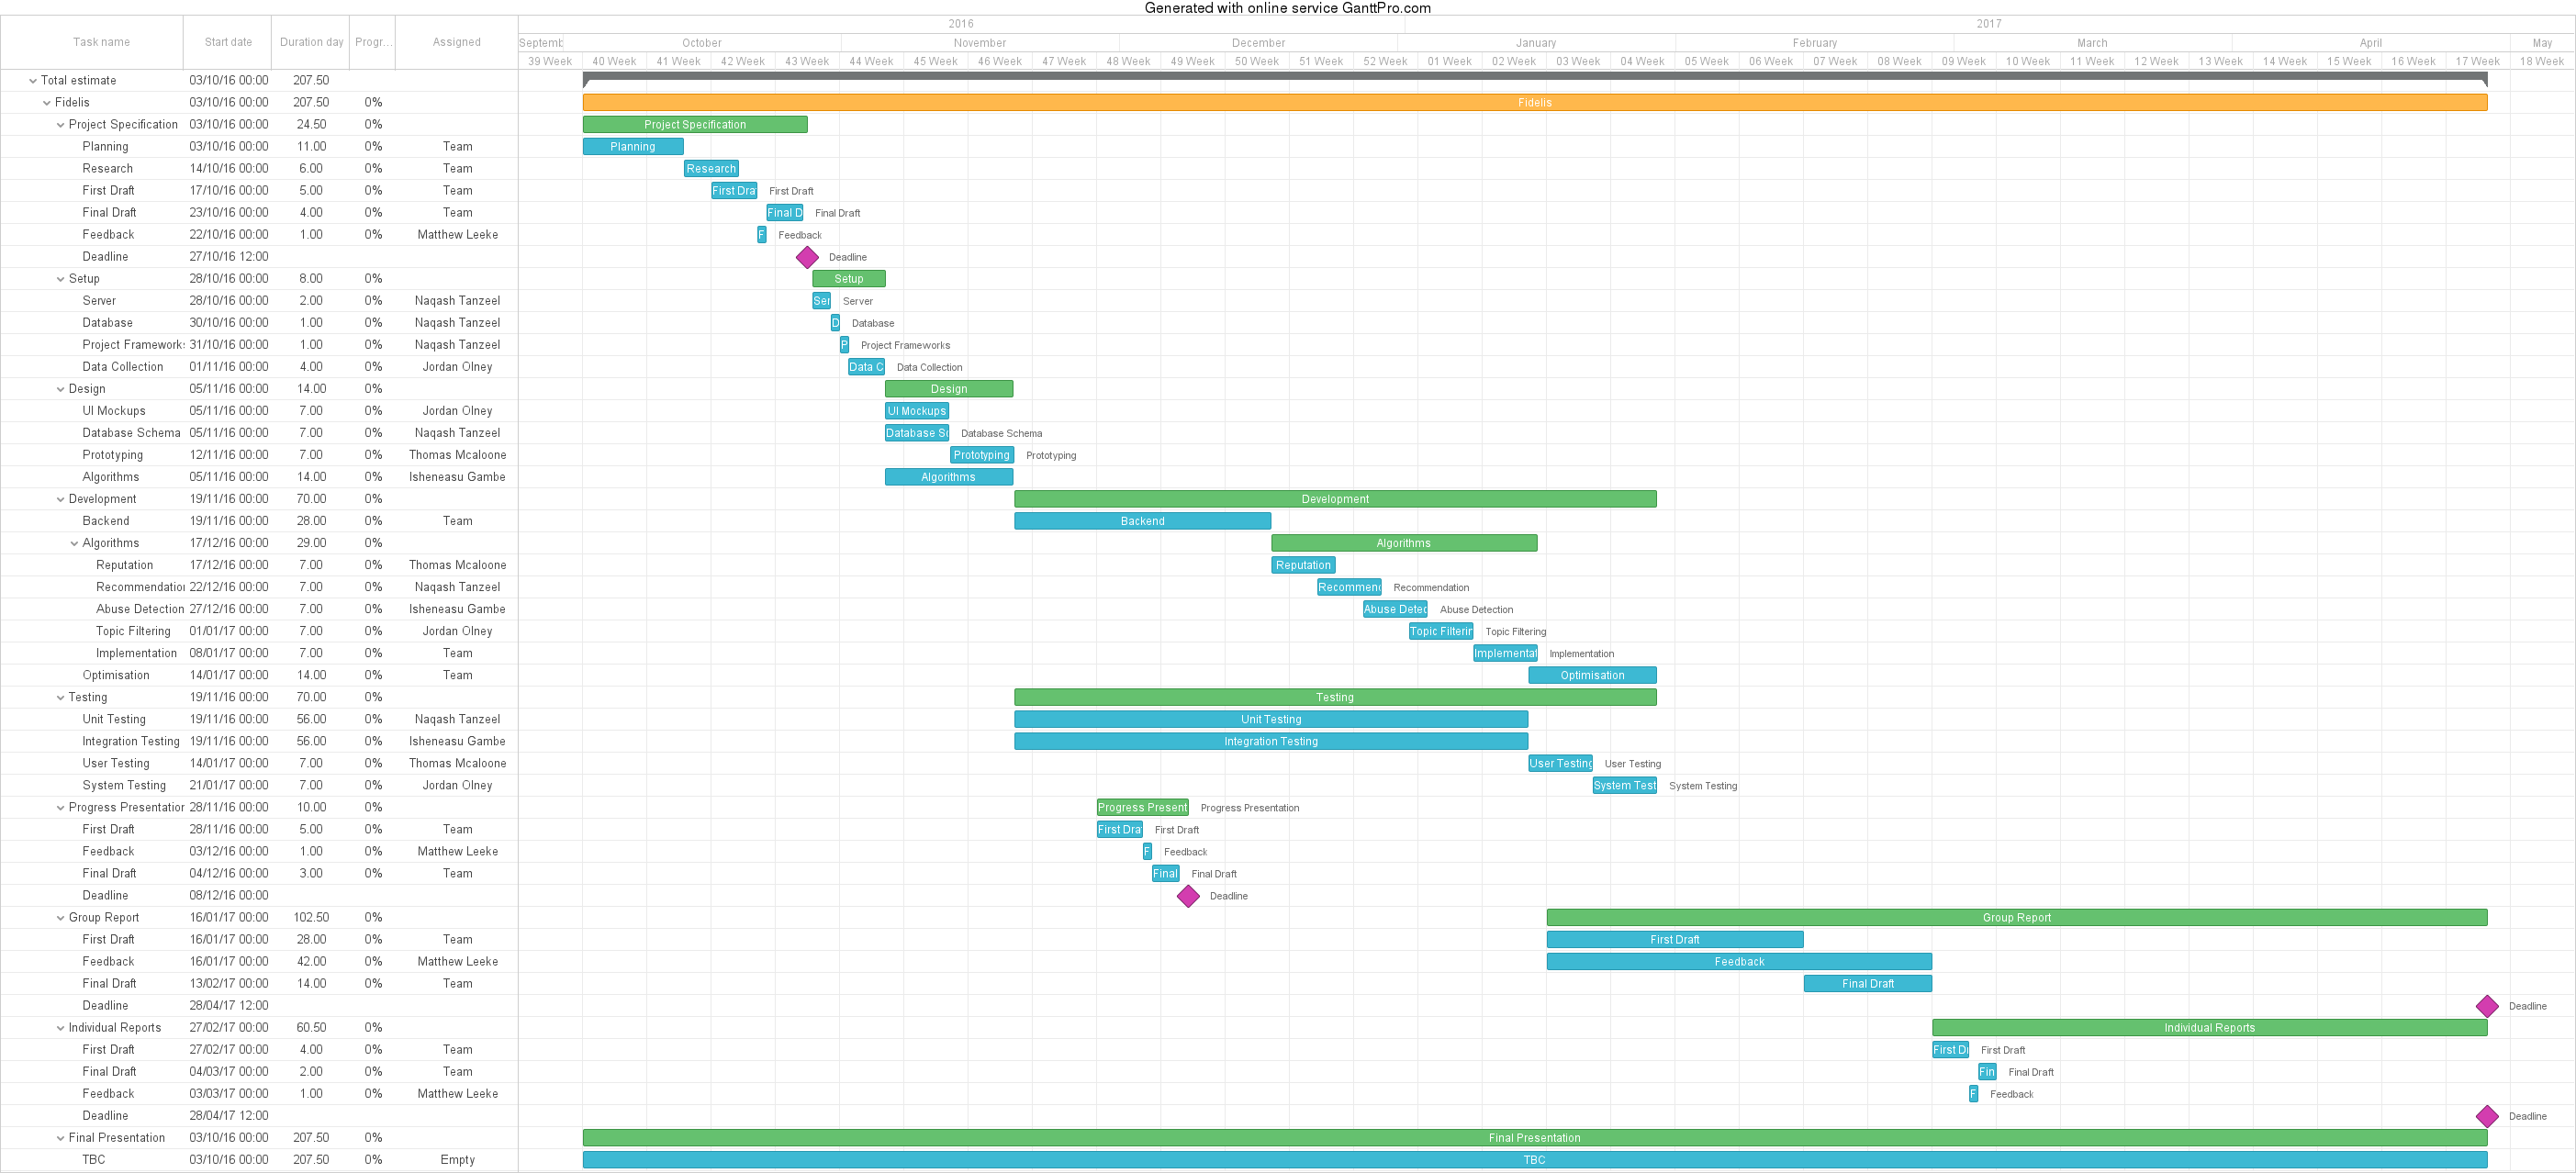
\includegraphics[width=1.0\textwidth]{Images/ProjectManagement/timeline}
  \caption{Project timeline} 
  \label{fig:timeline} 
\end{figure}

\section{Tools and Techniques}
\subsection{Development}
\subsection{Management}

\section{Risk Management}
Undertaking a project of this length, with the given time-scale and the nature of any software development project it was imperative that proper risk management be conducted to minimise major risks affecting project completion. Risks affecting developers, software, hardware, data and third party services were all considered and mitigated against.

\subsection{Developer}
Project developers are crucial to project success. As with any software development project, the importance in understanding and managing risks that may affect developers cannot be undervalued. One of the main risks affecting any developer is their ability to perform the tasks they are assigned to. Illness, commitments to other work assignments or an inability to complete a given task can severely hinder project progress. To prevent any such occurrence, all developers were paired so that in the event that developer A was unable to complete a task, developer B would be able to . Going beyond this, it was highly encouraged amongst the team to be aware of what other members were working on. This essentially meant that any developer was able to pick up tasks being handled by another developer. Additionally to this, effective communication channels were established within the team. This supported the idea of paired development as it made it easy for developers to work together, and also meant that potential issues were swiftly identified and dealt with.

\subsection{Hardware}
All development has been done using personal computers, so the only hardware relied upon during the project were these devices. Along with other work and personal use, each device was used heavily, and was therefore prone to failure. To mitigate against this, version control software was used to maintain functioning back-ups of all development work. Namely, Github was used for this purpose. Github allows ``snapshots'' of the functioning system to be taken, making data retrieval in the event of hardware failure very convenient and easily. In addition to this, each developer kept a copy of their work on the Computer Science Department lab machines. These two approaches covered the occurrence of single or complete device failure.

\subsection{Data}
Data security is important to any project where user data is collected. Exposing user data could leave the system and developers liable to penalties or criminal charges from relevant regulatory bodies so it is important to ensure that in the case that user data is exposed, safeguards are in place to protect both the users and developers. To avoid storing plain-text user credentials, they will be hashed before being stored in the database, making it almost impossible for anyone to decrypt the data within a reasonable period of time. During the registration process, minimal information is requested from the user. When registering, the only information requested from the user is their name and email address. This minimal approach on user information lessens the amount of sensitive data held on users. Password-protecting the database added an extra layer of database security, minimising the chances of unauthorised access to any of the data.

Another piece of data that needs to be protected is any content that is uploaded by the
user. Public user profiles are accessible to anyone on Fidelis, even to unregistered users. To provide users with the option of increased privacy, the user has the option to make their account private. This makes their content accessible only to their followers.

\subsection{Third Party Services}